% MSc dissertation example file, February 2022
%
% Leave one of the documentclass lines uncommented to match your degree.
% You may remove the logo option if it causes problems.
% Do not change any other options.
% \documentclass[logo,msc,adi]{infthesis}     % Adv Design Inf
% \documentclass[logo,msc,ai]{infthesis}      % AI
% \documentclass[logo,msc,cogsci]{infthesis}  % Cognitive Sci
% \documentclass[logo,msc,cs]{infthesis}      % Computer Sci
% \documentclass[logo,msc,cyber]{infthesis}   % Cyber Sec
% \documentclass[logo,msc,datasci]{infthesis} % Data Sci
% \documentclass[logo,msc,di]{infthesis}      % Design Inf
% \documentclass[logo,msc,dsti]{infthesis}    % Data Sci TI
% \documentclass[logo,msc,inf]{infthesis}     % Informatics
\documentclass[logo,msc]{infthesis}           % degree unspecified, do not change except to add your degree
%%%%%%%%%%%%%%%%%%%%%%%%
% Understand any problems and seek approval before assuming it's ok to remove ugcheck.
\usepackage{msccheck}

% Include any packages you need below, but don't include any that change the page
% layout or style of the dissertation. By including the ugcheck package above,
% you should catch most accidental changes of page layout though.

\usepackage{microtype} % recommended, but you can remove if it causes problems

% Content-support packages only; none changes the required page layout.
\usepackage{amsmath}
\usepackage{array}
\usepackage{booktabs}
\usepackage{calc}
\usepackage{hyperref}
\usepackage{longtable}
\usepackage{tabularx}
\usepackage{tikz}
\usetikzlibrary{positioning,arrows.meta,shapes.geometric,calc}

% Definitions emitted by the Markdown-to-LaTeX conversion.
\providecommand{\tightlist}{%
  \setlength{\itemsep}{0pt}\setlength{\parskip}{0pt}}

\begin{document}
\begin{preliminary}

\title{How Reliable Are LLMs as Cognitive Models?\\
\large A Systematic Evaluation of Prompt Sensitivity Across Decision-Making Tasks}

\author{TODO: insert author name}

\date{\today}

\abstract{
\textbf{TODO:} The supplied \texttt{final.md} does not yet contain an abstract.
Insert the final concise summary here without changing the surrounding template structure.
}

\maketitle

\newenvironment{ethics}
   {\begin{frontenv}{Research Ethics Approval}{\LARGE}}
   {\end{frontenv}\newpage}

\begin{ethics}
\textbf{Instructions:} \emph{Agree with your supervisor which
statement you need to include. Then delete the statement that you are not using,
and the instructions in italics.\\
\textbf{Either complete and include this statement:}}\\ % DELETE THESE INSTRUCTIONS
%
% IF ETHICS APPROVAL WAS REQUIRED:
This project obtained approval from the Informatics Research Ethics committee.\\
Ethics application number: ???\\
Date when approval was obtained: YYYY-MM-DD\\
%
\emph{[If the project required human participants, edit as appropriate, otherwise delete:]}\\ % DELETE THIS LINE
The participants' information sheet and a consent form are included in the appendix.\\
%
% IF ETHICS APPROVAL WAS NOT REQUIRED:
\textbf{\emph{Or include this statement:}}\\ % DELETE THIS LINE
This project was planned in accordance with the Informatics Research
Ethics policy. It did not involve any aspects that required approval
from the Informatics Research Ethics committee.

\standarddeclaration
\end{ethics}

\begin{acknowledgements}
\textbf{TODO:} Insert acknowledgements, or remove this optional environment.
\end{acknowledgements}

\tableofcontents
\end{preliminary}

% Dissertation body filled from the supplied final.md.
\hypertarget{introduction}{%
\chapter{Introduction}\label{introduction}}

\hypertarget{background-and-related-work}{%
\chapter{Background and Related Work}\label{background-and-related-work}}

\hypertarget{llms-as-objects-and-instruments-of-behavioural-research}{%
\section{LLMs as Objects and Instruments of Behavioural Research}\label{llms-as-objects-and-instruments-of-behavioural-research}}

\hypertarget{behavioural-similarity-cognitive-modelling-and-construct-validity}{%
\section{Behavioural Similarity, Cognitive Modelling, and Construct Validity}\label{behavioural-similarity-cognitive-modelling-and-construct-validity}}

\hypertarget{prompt-formulation-as-part-of-the-measurement-procedure}{%
\section{Prompt Formulation as Part of the Measurement Procedure}\label{prompt-formulation-as-part-of-the-measurement-procedure}}

\hypertarget{sequential-decision-tasks-as-behavioural-tests-of-llms}{%
\section{Sequential Decision Tasks as Behavioural Tests of LLMs}\label{sequential-decision-tasks-as-behavioural-tests-of-llms}}

\hypertarget{behavioural-reliability-as-a-multidimensional-evaluation-problem}{%
\section{Behavioural Reliability as a Multidimensional Evaluation Problem}\label{behavioural-reliability-as-a-multidimensional-evaluation-problem}}

\hypertarget{cross-model-variation-and-reproducibility}{%
\section{Cross-Model Variation and Reproducibility}\label{cross-model-variation-and-reproducibility}}

\hypertarget{multilingual-evaluation-and-cross-language-behaviour}{%
\section{Multilingual Evaluation and Cross-Language Behaviour}\label{multilingual-evaluation-and-cross-language-behaviour}}

\hypertarget{synthesis-and-positioning-of-the-present-study}{%
\section{Synthesis and Positioning of the Present Study}\label{synthesis-and-positioning-of-the-present-study}}

\hypertarget{method}{%
\chapter{Method}\label{method}}

\hypertarget{study-design-and-scope}{%
\section{Study Design and Scope}\label{study-design-and-scope}}

\begin{figure}[htbp]
    \centering
    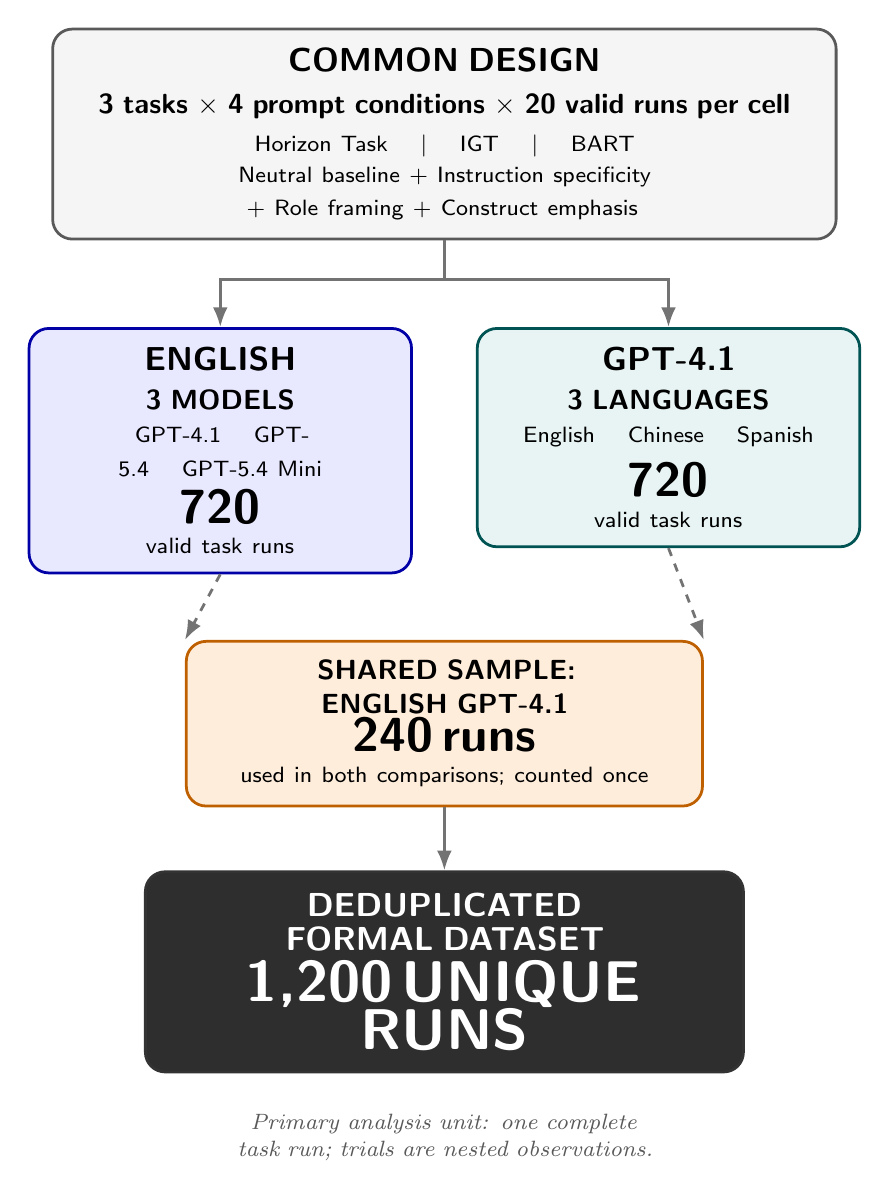
\begin{tikzpicture}[
        font=\sffamily,
        >=Latex,
        arrow/.style={-{Latex[length=2.5mm]}, line width=1pt, draw=black!55},
        branch/.style={
            rounded corners=2.5mm,
            line width=1pt,
            align=center,
            text width=0.36\textwidth,
            minimum height=25mm,
            inner sep=7pt
        }
    ]

    % Step 1: common structure
    \node[
        draw=black!65,
        fill=black!4,
        rounded corners=2.5mm,
        line width=1pt,
        align=center,
        text width=0.78\textwidth,
        inner sep=7pt
    ] (common) {
        {\large\bfseries COMMON DESIGN}\\[3pt]
        {\bfseries 3 tasks $\times$ 4 prompt conditions $\times$ 20 valid runs per cell}\\[2pt]
        {\footnotesize Horizon Task \quad $\vert$ \quad IGT \quad $\vert$ \quad BART}\\[-1pt]
        {\footnotesize Neutral baseline $+$ Instruction specificity $+$ Role framing $+$ Construct emphasis}
    };

    % Step 2: two comparison arms
    \node[
        branch,
        draw=blue!65!black,
        fill=blue!9,
        below left=11mm and 4mm of common.south
    ] (modelarm) {
        {\large\bfseries ENGLISH}\\[2pt]
        {\bfseries 3 MODELS}\\
        {\footnotesize GPT-4.1 \quad GPT-5.4 \quad GPT-5.4 Mini}\\[5pt]
        {\fontsize{18}{20}\selectfont\bfseries 720}\\[-1pt]
        {\footnotesize valid task runs}
    };

    \node[
        branch,
        draw=teal!65!black,
        fill=teal!9,
        below right=11mm and 4mm of common.south
    ] (languagearm) {
        {\large\bfseries GPT-4.1}\\[2pt]
        {\bfseries 3 LANGUAGES}\\
        {\footnotesize English \quad Chinese \quad Spanish}\\[5pt]
        {\fontsize{18}{20}\selectfont\bfseries 720}\\[-1pt]
        {\footnotesize valid task runs}
    };

    \draw[arrow] (common.south) -- ++(0,-5mm) -| (modelarm.north);
    \draw[arrow] (common.south) -- ++(0,-5mm) -| (languagearm.north);

    % Step 3: overlap that must be counted once
    \node[
        draw=orange!75!black,
        fill=orange!14,
        rounded corners=2.5mm,
        line width=1pt,
        align=center,
        text width=0.50\textwidth,
        inner sep=7pt,
        below=10mm of $(modelarm.south)!0.5!(languagearm.south)$
    ] (shared) {
        {\bfseries SHARED SAMPLE: ENGLISH GPT-4.1}\\[2pt]
        {\fontsize{16}{18}\selectfont\bfseries 240 runs}\\[-1pt]
        {\footnotesize used in both comparisons; counted once}
    };

    \draw[arrow, dashed] (modelarm.south) -- (shared.north west);
    \draw[arrow, dashed] (languagearm.south) -- (shared.north east);

    % Step 4: deduplicated total
    \node[
        draw=black!80,
        fill=black!82,
        text=white,
        rounded corners=2.5mm,
        line width=1pt,
        align=center,
        text width=0.58\textwidth,
        inner sep=8pt,
        below=8mm of shared
    ] (total) {
        {\large\bfseries DEDUPLICATED FORMAL DATASET}\\[3pt]
        {\fontsize{22}{24}\selectfont\bfseries 1,200 UNIQUE RUNS}
    };

    \draw[arrow] (shared.south) -- (total.north);

    \node[
        below=4mm of total,
        align=center,
        text width=0.72\textwidth,
        font=\footnotesize\itshape,
        text=black!65
    ] {
        Primary analysis unit: one complete task run; trials are nested observations.
    };

    \end{tikzpicture}
    \caption{Study design and deduplicated data structure. The English GPT-4.1 runs are shared across the two comparison arms and therefore counted only once.}
    \label{fig:study_design_scope}
\end{figure}

\hypertarget{models-and-api-configuration}{%
\section{Models and API Configuration}\label{models-and-api-configuration}}

\begin{table}[htbp]
    \centering
    \caption{Model identifiers and formal data-collection periods.}
    \label{tab:model_identifiers}
    \begin{tabularx}{\textwidth}{
        >{\raggedright\arraybackslash}p{2.3cm}
        >{\raggedright\arraybackslash}X
        >{\raggedright\arraybackslash}X
        >{\raggedright\arraybackslash}p{2.8cm}
    }
        \toprule
        \textbf{Model} &
        \textbf{Requested identifier} &
        \textbf{Resolved identifier} &
        \textbf{Collection period} \\
        \midrule
        GPT-4.1
        & \texttt{gpt-4.1-2025-04-14}
        & \texttt{gpt-4.1-2025-04-14}
        & English: 8--13 July 2026; zh-CN: 3--5 August 2026; es: 5--7 August 2026 \\

        GPT-5.4
        & \texttt{gpt-5.4}
        & \texttt{gpt-5.4-2026-03-05}
        & 30--31 July 2026 \\

        GPT-5.4 Mini
        & \texttt{gpt-5.4-mini}
        & \texttt{gpt-5.4-mini-2026-03-17}
        & 1 August 2026 \\
        \bottomrule
    \end{tabularx}
\end{table}

\hypertarget{decision-making-tasks}{%
\section{Decision-Making Tasks}\label{decision-making-tasks}}

\hypertarget{horizon-task}{%
\subsection{Horizon Task}\label{horizon-task}}

\hypertarget{iowa-gambling-task}{%
\subsection{Iowa Gambling Task}\label{iowa-gambling-task}}

\hypertarget{balloon-analogue-risk-task}{%
\subsection{Balloon Analogue Risk Task}\label{balloon-analogue-risk-task}}

\hypertarget{prompt-construction-and-validation}{%
\section{Prompt Construction and Validation}\label{prompt-construction-and-validation}}

\hypertarget{prompt-conditions}{%
\subsection{Prompt Conditions}\label{prompt-conditions}}

\hypertarget{prompt-provenance-validation-and-freezing}{%
\subsection{Prompt Provenance, Validation, and Freezing}\label{prompt-provenance-validation-and-freezing}}

\hypertarget{multilingual-prompt-construction-and-validation}{%
\subsection{Multilingual Prompt Construction and Validation}\label{multilingual-prompt-construction-and-validation}}

\hypertarget{experimental-procedure-and-data-quality}{%
\section{Experimental Procedure and Data Quality}\label{experimental-procedure-and-data-quality}}

\begin{figure}[htbp]
    \centering
    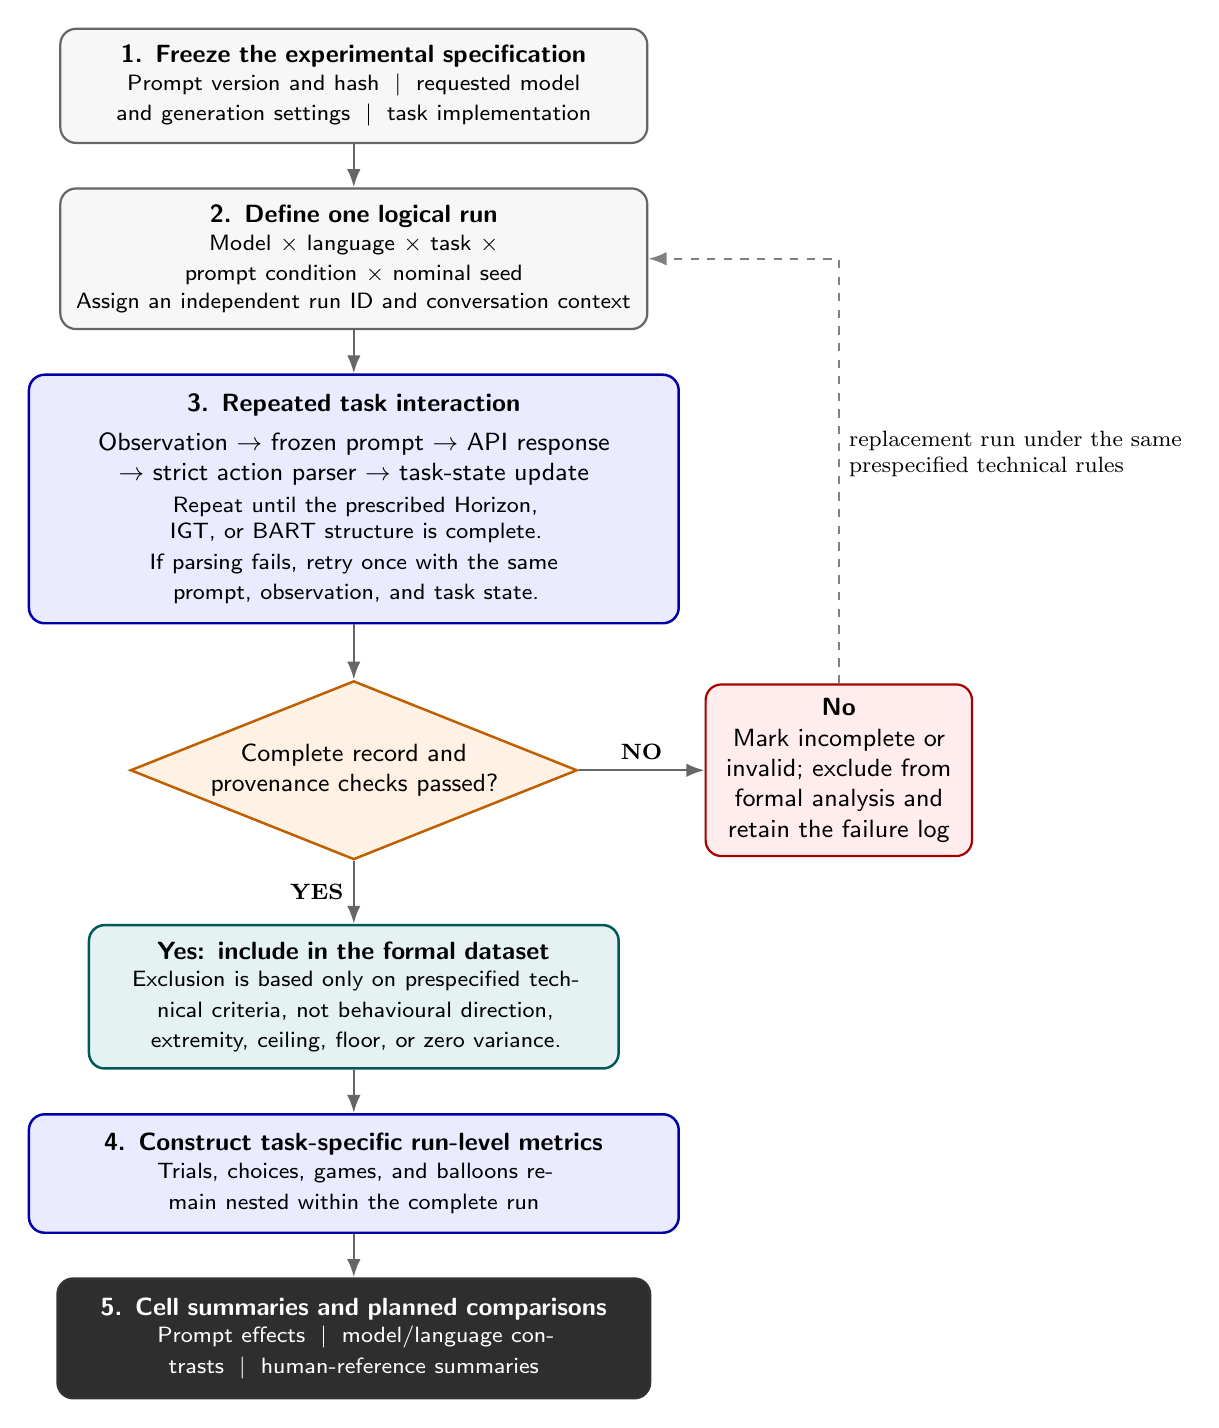
\begin{tikzpicture}[
        font=\sffamily\small,
        node distance=5.5mm and 13mm,
        >=Latex,
        flow/.style={-{Latex[length=2.3mm]}, line width=0.9pt, draw=black!60},
        return/.style={-{Latex[length=2.3mm]}, line width=0.8pt, dashed, draw=black!50},
        box/.style={
            rectangle,
            rounded corners=2mm,
            draw=black!60,
            fill=black!3,
            line width=0.8pt,
            align=center,
            text width=0.58\textwidth,
            inner sep=6pt
        },
        process/.style={
            rectangle,
            rounded corners=2mm,
            draw=blue!65!black,
            fill=blue!8,
            line width=0.9pt,
            align=center,
            text width=0.64\textwidth,
            inner sep=7pt
        },
        decision/.style={
            diamond,
            aspect=2.5,
            draw=orange!75!black,
            fill=orange!11,
            line width=0.9pt,
            align=center,
            inner sep=1.5pt,
            text width=0.30\textwidth
        },
        success/.style={
            rectangle,
            rounded corners=2mm,
            draw=teal!70!black,
            fill=teal!10,
            line width=0.9pt,
            align=center,
            text width=0.52\textwidth,
            inner sep=6pt
        },
        failure/.style={
            rectangle,
            rounded corners=2mm,
            draw=red!65!black,
            fill=red!7,
            line width=0.8pt,
            align=center,
            text width=0.25\textwidth,
            inner sep=5pt
        }
    ]

    \node[box] (freeze) {
        \textbf{1. Freeze the experimental specification}\\[-1pt]
        {\footnotesize Prompt version and hash \;$\vert$\; requested model and generation settings \;$\vert$\; task implementation}
    };

    \node[box, below=of freeze] (run) {
        \textbf{2. Define one logical run}\\[-1pt]
        {\footnotesize Model $\times$ language $\times$ task $\times$ prompt condition $\times$ nominal seed}\\[-1pt]
        {\footnotesize Assign an independent run ID and conversation context}
    };

    \node[process, below=of run] (loop) {
        \textbf{3. Repeated task interaction}\\[3pt]
        Observation $\rightarrow$ frozen prompt $\rightarrow$ API response
        $\rightarrow$ strict action parser $\rightarrow$ task-state update\\[2pt]
        {\footnotesize Repeat until the prescribed Horizon, IGT, or BART structure is complete.\\
        If parsing fails, retry once with the same prompt, observation, and task state.}
    };

    \node[decision, below=7mm of loop] (valid) {
        Complete record and provenance checks passed?
    };

    \node[failure, right=16mm of valid] (invalid) {
        \textbf{No}\\
        Mark incomplete or invalid; exclude from formal analysis and retain the failure log
    };

    \node[success, below=8mm of valid] (include) {
        \textbf{Yes: include in the formal dataset}\\[-1pt]
        {\footnotesize Exclusion is based only on prespecified technical criteria, not behavioural direction, extremity, ceiling, floor, or zero variance.}
    };

    \node[process, below=of include] (metrics) {
        \textbf{4. Construct task-specific run-level metrics}\\[-1pt]
        {\footnotesize Trials, choices, games, and balloons remain nested within the complete run}
    };

    \node[
        rectangle,
        rounded corners=2mm,
        draw=black!80,
        fill=black!82,
        text=white,
        line width=0.9pt,
        align=center,
        text width=0.58\textwidth,
        inner sep=7pt,
        below=of metrics
    ] (analysis) {
        \textbf{5. Cell summaries and planned comparisons}\\[-1pt]
        {\footnotesize Prompt effects \;$\vert$\; model/language contrasts \;$\vert$\; human-reference summaries}
    };

    \draw[flow] (freeze) -- (run);
    \draw[flow] (run) -- (loop);
    \draw[flow] (loop) -- (valid);
    \draw[flow] (valid) -- node[left, font=\footnotesize\bfseries] {YES} (include);
    \draw[flow] (valid.east) -- node[above, font=\footnotesize\bfseries] {NO} (invalid.west);
    \draw[flow] (include) -- (metrics);
    \draw[flow] (metrics) -- (analysis);

    \draw[return] (invalid.north) |- node[pos=0.27, right, font=\footnotesize, align=left]
        {replacement run under the same\\prespecified technical rules} (run.east);

    \end{tikzpicture}
    \caption{Workflow for task execution, technical validation, and inclusion in the formal analysis.}
    \label{fig:experimental_workflow}
\end{figure}

\hypertarget{run-procedure}{%
\subsection{Run procedure}\label{run-procedure}}

\hypertarget{response-parsing-and-quality-control}{%
\subsection{Response parsing and quality control}\label{response-parsing-and-quality-control}}

\hypertarget{human-reference-data}{%
\section{Human Reference Data}\label{human-reference-data}}

\hypertarget{statistical-analysis}{%
\section{Statistical Analysis}\label{statistical-analysis}}

\hypertarget{behavioural-metrics}{%
\subsection{Behavioural Metrics}\label{behavioural-metrics}}

\begin{longtable}[]{@{}
  >{\raggedright\arraybackslash}p{(\columnwidth - 4\tabcolsep) * \real{0.0761}}
  >{\raggedright\arraybackslash}p{(\columnwidth - 4\tabcolsep) * \real{0.2717}}
  >{\raggedright\arraybackslash}p{(\columnwidth - 4\tabcolsep) * \real{0.6522}}@{}}
\toprule
\begin{minipage}[b]{\linewidth}\raggedright
Task
\end{minipage} & \begin{minipage}[b]{\linewidth}\raggedright
Metric
\end{minipage} & \begin{minipage}[b]{\linewidth}\raggedright
Definition for one participant/run
\end{minipage} \\
\midrule
\endhead
Horizon & Information-seeking choice rate (data field: \texttt{directed\_exploration}) & Proportion of unequal-information first free choices directed toward the less-observed option \\
Horizon & Horizon-related exploration change (data field: \texttt{horizon\_effect}) & Horizon 6 minus Horizon 1 first-free-choice exploration rate; both information conditions are included and ties in observed means are excluded \\
Horizon & Random exploration effect & Horizon-specific decision-noise difference estimated by the hierarchical logistic model of first free choices \\
IGT & Advantageous choice rate & Proportion of the 100 trials on which deck C or D is selected \\
IGT & Post-loss switching rate & Proportion of eligible trials followed by a switch when the preceding trial has a negative signed loss component \\
BART & Adjusted average pumps & Mean number of pumps across balloons that do not explode \\
BART & Explosion rate & Proportion of all balloons that explode \\
BART & Post-explosion adjustment & Mean difference between pumps on the balloon following an explosion and pumps on the exploded balloon \\
\bottomrule
\end{longtable}

\hypertarget{prompt-effects}{%
\subsection{Prompt Effects}\label{prompt-effects}}

\hypertarget{cross-model-comparisons}{%
\subsection{Cross-Model Comparisons}\label{cross-model-comparisons}}

\hypertarget{cross-language-comparisons}{%
\subsection{Cross-Language Comparisons}\label{cross-language-comparisons}}

\hypertarget{prompt-sensitivity-index}{%
\subsection{Prompt Sensitivity Index}\label{prompt-sensitivity-index}}

\hypertarget{human-reference-comparisons}{%
\subsection{Human-Reference Comparisons}\label{human-reference-comparisons}}

\hypertarget{uncertainty-and-robustness-analyses}{%
\subsection{Uncertainty and Robustness Analyses}\label{uncertainty-and-robustness-analyses}}

\hypertarget{reproducibility}{%
\section{Reproducibility}\label{reproducibility}}

\hypertarget{results-and-discussion}{%
\chapter{Results and Discussion}\label{results-and-discussion}}

\hypertarget{conclusion-and-future-work}{%
\chapter{Conclusion and Future Work}\label{conclusion-and-future-work}}

% The supplied final.md contains an empty Bibliography section.
% Insert the verified bibliography here when it is available.

% You may delete everything from \appendix up to \end{document} if you don't need it.
% No appendix content was present in the supplied final.md, so no appendix is
% instantiated in this version.

\end{document}

